%% PNAStmpl.tex
%% Template file to use for PNAS articles prepared in LaTeX
%% Version: Apr 14, 2008


%%%%%%%%%%%%%%%%%%%%%%%%%%%%%%
%% BASIC CLASS FILE
%% PNAStwo for two column articles is called by default.
%% Uncomment PNASone for single column articles. One column class
%% and style files are available upon request from pnas@nas.edu.
%% (uncomment means get rid of the '%' in front of the command)

%\documentclass{pnasone}
\documentclass{pnastwo}

%%%%%%%%%%%%%%%%%%%%%%%%%%%%%%
%% Changing position of text on physical page:
%% Since not all printers position
%% the printed page in the same place on the physical page,
%% you can change the position yourself here, if you need to:

% \advance\voffset -.5in % Minus dimension will raise the printed page on the
                         %  physical page; positive dimension will lower it.

%% You may set the dimension to the size that you need.

%%%%%%%%%%%%%%%%%%%%%%%%%%%%%%
%% OPTIONAL GRAPHICS STYLE FILE

%% Requires graphics style file (graphicx.sty), used for inserting
%% .eps files into LaTeX articles.
%% Note that inclusion of .eps files is for your reference only;
%% when submitting to PNAS please submit figures separately.

%% Type into the square brackets the name of the driver program
%% that you are using. If you don't know, try dvips, which is the
%% most common PC driver, or textures for the Mac. These are the options:

% [dvips], [xdvi], [dvipdf], [dvipdfm], [dvipdfmx], [pdftex], [dvipsone],
% [dviwindo], [emtex], [dviwin], [pctexps], [pctexwin], [pctexhp], [pctex32],
% [truetex], [tcidvi], [vtex], [oztex], [textures], [xetex]

%\usepackage[dvips]{graphicx}

%%%%%%%%%%%%%%%%%%%%%%%%%%%%%%
%% OPTIONAL POSTSCRIPT FONT FILES

%% PostScript font files: You may need to edit the PNASoneF.sty
%% or PNAStwoF.sty file to make the font names match those on your system.
%% Alternatively, you can leave the font style file commands commented out
%% and typeset your article using the default Computer Modern
%% fonts (recommended). If accepted, your article will be typeset
%% at PNAS using PostScript fonts.

% Choose PNASoneF for one column; PNAStwoF for two column:
%\usepackage{PNASoneF}
\usepackage{PNAStwoF}

%%%%%%%%%%%%%%%%%%%%%%%%%%%%%%
%% ADDITIONAL OPTIONAL STYLE FILES

%% The AMS math files are commonly used to gain access to useful features
%% like extended math fonts and math commands.

\usepackage{amssymb,amsfonts,amsmath}

%\usepackage{subcaption}
\graphicspath{ {paper_figures2/} }

\usepackage{tikz}

%\usepackage{sansmath}

%\usepackage[font={sf, small}]{caption}

%%%%%%%%%%%%%%%%%%%%%%%%%%%%%%
%% OPTIONAL MACRO FILES
%% Insert self-defined macros here.
%% \newcommand definitions are recommended; \def definitions are supported

%\newcommand{\mfrac}[2]{\frac{\displaystyle #1}{\displaystyle #2}}
%\def\s{\sigma}

\DeclareMathSizes{9}{8}{7}{7}

\DeclareMathOperator*{\argmin}{arg\,min}

\makeatletter
\newcommand{\customlabel}[2]{%
\protected@write \@auxout {}{\string \newlabel {#1}{{#2}{}}}}
\makeatother

%%%%%%%%%%%%%%%%%%%%%%%%%%%%%%
%% Don't type in anything in the following section:
%%%%%%%%%%%%
%% For PNAS Only:
\contributor{Submitted to Proceedings
of the National Academy of Sciences of the United States of America}
\url{www.pnas.org/cgi/doi/10.1073/pnas.0709640104}
\copyrightyear{2008}
\issuedate{Issue Date}
\volume{Volume}
\issuenumber{Issue Number}
%%%%%%%%%%%%

\begin{document}

%%%%%%%%%%%%%%%%%%%%%%%%%%%%%%


%% For titles, only capitalize the first letter
%% \title{Almost sharp fronts for the surface quasi-geostrophic equation}

\title{Temporal ordering and registration of images in studies of developmental dynamics}

%% Enter authors via the \author command.
%% Use \affil to define affiliations.
%% (Leave no spaces between author name and \affil command)

%% Note that the \thanks{} command has been disabled in favor of
%% a generic, reserved space for PNAS publication footnotes.

%% \author{<author name>
%% \affil{<number>}{<Institution>}} One number for each institution.
%% The same number should be used for authors that
%% are affiliated with the same institution, after the first time
%% only the number is needed, ie, \affil{number}{text}, \affil{number}{}
%% Then, before last author ...
%% \and
%% \author{<author name>
%% \affil{<number>}{}}

%% For example, assuming Garcia and Sonnery are both affiliated with
%% Universidad de Murcia:
%% \author{Roberta Graff\affil{1}{University of Cambridge, Cambridge,
%% United Kingdom},
%% Javier de Ruiz Garcia\affil{2}{Universidad de Murcia, Bioquimica y Biologia
%% Molecular, Murcia, Spain}, \and Franklin Sonnery\affil{2}{}}

\author{Carmeline~J.~Dsilva\affil{1}{Department of Chemical and Biological Engineering, Princeton University, Princeton, New Jersey, USA},
Bomyi~Lim\affil{1}{},
Thomas~J.~Levario\affil{2}{School of Chemical and Biomolecular Engineering, Georgia Institute of Technology, Atlanta, Georgia, USA},
Hang~Lu\affil{2}{},
Amit~Singer\affil{3}{Department of Mathematics, Princeton University, Princeton, New Jersey, USA} \affil{4}{Program in Applied and Computational Mathematics, Princeton University, Princeton, New Jersey, USA},
Stanislav~Y.~Shvartsman\affil{1}{} \affil{5}{Lewis-Sigler Institute for Integrative Genomics, Princeton University, Princeton, New Jersey, USA},
\and
Ioannis~G.~Kevrekidis\affil{1}{} \affil{4}{Program in Applied and Computational Mathematics, Princeton University, Princeton, New Jersey, USA}}

\contributor{Submitted to Proceedings of the National Academy of Sciences
of the United States of America}

%% The \maketitle command is necessary to build the title page.
\maketitle

%%%%%%%%%%%%%%%%%%%%%%%%%%%%%%%%%%%%%%%%%%%%%%%%%%%%%%%%%%%%%%%%
\begin{article}

\begin{abstract}
In studies of development, researchers are often presented with cross-sectional data, where each data point is a sample from a population fixed at a 
%slightly 
different developmental time.
%
The goal is then to temporally order the data to reconstruct the developmental dynamics.
%
Data points in the form of two-dimensional image must first be registered before they can be temporally ordered.
%
When such data sets are large, noisy, and/or if the developmental changes are subtle, these tasks can be difficult to perform by hand.
%
We present an automated approach to registering {\it and} temporally ordering cross-sectional data sets of images.
%
The mathematical techniques (vector diffusion maps) are applicable to a wide variety of data sets and
require little {\it a priori} knowledge of the image features or the developmental dynamics.
%
%Furthermore, these techniques can separate multiple trajectories within the same data set.
%
Furthermore, the approach can detect multiple sources of variability 
and thus help visualize multiple trajectories within a data set.
%
We demonstrate the utility of these methods using a collection of images from a study of {\it Drosophila} embryogenesis.
\end{abstract}


%% When adding keywords, separate each term with a straight line: |
\keywords{temporal ordering | image registration | vector diffusion maps}

%% Optional for entering abbreviations, separate the abbreviation from
%% its definition with a comma, separate each pair with a semicolon:
%% for example:
%% \abbreviations{SAM, self-assembled monolayer; OTS,
%% octadecyltrichlorosilane}

% \abbreviations{}

%% The first letter of the article should be drop cap: \dropcap{}
%\dropcap{I}n this article we study the evolution of ''almost-sharp'' fronts

%% Enter the text of your article beginning here and ending before
%% \begin{acknowledgements}
%% Section head commands for your reference:
%% \section{}
%% \subsection{}
%% \subsubsection{}



\dropcap{E}xperimental studies of developmental dynamics fall in two broadly defined categories: longitudinal and cross-sectional \cite{diggle2002analysis}.
%
In longitudinal studies, developmental progress is monitored over time for the same embryo.
%
In a cross-sectional study, developmental dynamics must be reconstructed from multiple embryos, each of which contributes only a single snapshot of a chemical or morphological process along its developmental trajectory.
%
Both of these sampling schemes have their advantages and limitations, and both are extensively used by biologists.
%%%
%%%YGK sounds condescending
%%%
%
Here we focus on cross-sectional studies, which have a time-honored history and still present the only option for most organisms.
%%%
%%%YGK  one or two refs ?
%%%
%
In a typical cross-sectional study, a group of embryos is fixed using a procedure that arrests their development and stained with chemicals that visualize a handful of cellular processes.
%
Fixed embryos are then imaged using any given number of microscopy techniques.
%
Recent advances in large-scale 
%%%
%%%YGK  large scale ? high throughput
%%%
physical manipulation and imaging of embryos produce rapidly increasing volumes of cross-sectional data, in which every embryo is observed at a different developmental time point but also at a different geometric orientation.  
%
Importantly, the ``age'' of any given embryo arrested in its development is not quantitatively known; typically what is known is 
a certain time window to which a collection of embryos belongs.
%to high accuracy.
%
Furthermore, each embryo appears at an arbitrary translation and rotation within the image frame (see {\it SI Appendix}). 
%
In order to recover the developmental dynamics from such data sets, snapshots of different embryos must be spatially aligned or {\em registered} to factor out the relevant geometric symmetries (e.g., translations and rotations), and then ordered in time.
%
We show how existing dimensionality reduction algorithms can automate, greatly accelerate {\it and combine} both of these tasks.

An example where 
temporal ordering and registration of images can be done manually
because the number of images is small and the differences between them are visually apparent is shown
in Figure~\ref{fig:fish}: a caricature of fish development which illustrates the processes of growth and patterning.
%
In this case, temporal ordering can be accomplished by arranging the fish by size, which is monotonic with the developmental progress.
%
Image registration is based on obvious morphological landmarks, such as the position of head and fins.
%
In contrast to this simple illustration, real data poses nontrivial challenges for both registration and temporal ordering.
%
In general, the landmarks needed for registration (here the heads and fins) as well as the attributes which can be used to order the data (such as the body length) are not known {\it a priori}.
%
Additional challenges arise from embryo-to-embryo variability, sample size, and measurement noise.

\begin{figure}[t]
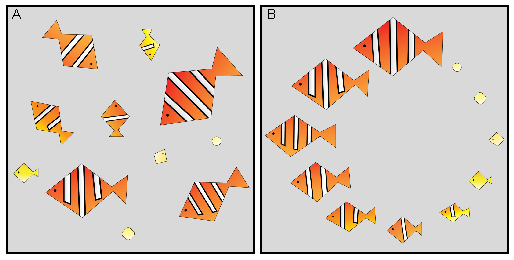
\includegraphics[width=8.7cm]{fig1}
\caption{Caricature illustrating the tasks of image registration and temporal ordering. {\xfigtextfontit (A)} Fish, each in a different orientation and a different stage of development. {\xfigtextfontit (B)} Fish, now rotationally registered and temporally ordered. For this caricature, the registration and ordering is easy to do ``by hand" because the data set is small and the developmental changes are easy to recognize.}
%\label{fig:fish}
\customlabel{fig:fish}{1}
\customlabel{subfig:fish_unordered}{\ref{fig:fish}{\it A}}
\customlabel{subfig:fish_ordered}{\ref{fig:fish}{\it B}}
\end{figure}

%%%YGK put an arrow in the disc

We show how recently developed dimensionality reduction techniques can successfully address these challenges and reveal developmental trajectories from collections of unregistered and unordered imaging data.
%
Image registration has been studied in a variety of contexts \cite{zitova2003image, rowley1998rotation, hajnal2010medical, greenspan1994rotation, zhao2003face}, and so have dimensionality reduction techniques \cite{Belkin2003, coifman2005geometric, coifman2006geometric, tenenbaum2000global, roweis2000nonlinear} and their applications \cite{anavy2014blind, trapnell2014dynamics,gupta2008extracting, qiu2011discovering, kafri2013dynamics}, especially in the last decade.
%
Here, we use a manifold learning algorithm \cite{singer2012vector} for high-dimensional imaging data.% which both factors out geometric symmetries to register the images and extracts low-dimensional structure in the imaging data set.
%
Such techniques have been used for data mining in 
applications ranging from analysis of cryo-electron microscopy images of individual molecules to face recognition; here they are adapted
for simultaneous registration and temporal ordering of imaging data from cross-sectional studies of developmental dynamics, with the main objective of revealing stereotypic developmental trajectories.
%
We analyze three data sets from a study of {\it Drosophila} embryogenesis, one of the best experimental models for studies of developmental dynamics.
%
The first data set, shown in Figure~\ref{subfig:raw_data1}, is relatively simple and will allow us to both illustrate and validate this approach.
%
In the second data set, shown in Figure~\ref{subfig:raw_data2}, the dynamics are significantly more complex.
%
Here, we will show that we can recover a trajectory that is qualitatively consistent with current knowledge.
%
The third set consists of data collected from both wild type and mutant embryos, and joint processing of the data will help to visualize the different sources of variability along distinct developmental paths.

%\begin{itemize}
%\item Imaging data is becoming increasingly prevalent in biology research.
%
%\item General motivation about biology data ...
%
%\item Need methods to organize data, visualize, ...
%
%\item REDUCTION is important, reduction because of symmetry and reduction because of content
%
%\item There are a bunch of recent techniques- some established (like dmaps), some very fresh, like synchronization or VDMaps,  that have had their own reasons to be developed but they are as if tailor made for what we would want to do
%\end{itemize}


\section{Results and Discussion}

\subsection{Vector diffusion maps for registration and temporal ordering}

%%%YGK  when I read this I think of Eiffel tower pictures, not of ours - there is a transition... careful where we do it.
%
Our goal is to organize data sets from cross-sectional studies of developmental processes in a meaningful and informative way.
%
%We will show that dimensionality reduction algorithms can simultaneously register and temporally order the images to give us a meaningful picture of the underlying developmental dynamics.
%
Our approach is based on vector diffusion maps \cite{singer2012vector}, a general technique developed for data sets which contain two types of sources of variability:
geometric symmetries (such as translations and rotations of the images due to the experimental setup) which one would like to factor out, 
and ``additional" directions of variability (such as temporal dynamics) which one wants to uncover.
%
Vector diffusion maps combine two algorithms, {\em angular synchronization} \cite{singer2011angular} for image registration and {\em diffusion maps} \cite{coifman2005geometric} for extracting intrinsic low-dimensional structure in data, into a single computation that allows us to simultaneously register and temporally order our images.
%

Vector diffusion maps has been used to classify images from cryo-electron microscopy (cryo-EM) experiments, where each image is a projection of a randomly oriented molecule.
%
%%%YGK to imply which rotations we need to have discussed it above
%%
Here, we will use the algorithm to register images of {\it Drosophila} embryos with respect to rotations and translations, as well as uncover the main direction of variability {\it after} removing translational and rotational symmetries.
%
We assume that, in this set of images, this main direction of variability is parameterized by the developmental time of each embryo, so taht uncovering this direction will allow us to recover the developmental dynamics.
%
Unlike the noise in the cryo-EM application, which is approximately Gaussian and arises from the measurement instrument, the noise in our experiments arises primarily from interembryo variability and does not have a known simple structure.

%%%somewhere I want a sentence that says this is for general symmetry groups of some kind, and HERE it is for..... (maybe in SI)
Angular synchronization uses pairwise alignment information to register a set of images in a globally consistent way.
%
A schematic illustration is shown in Figure~\ref{subfig:synch1}, where each image is depicted as a vector, and the goal is to align the set of vectors.
%
We first compute the angles needed to align pairs of vectors (or images).
%
In general, this requires no template function \cite{ahuja2007template} or image landmarks \cite{ian1998statistical}; 
however, when the images are noisy, some pairwise alignments may be inaccurate.
%
Using the alignment angles between all pairs of vectors (or images), angular synchronization finds the set of rotation angles (one angle for each vector) most consistent with all pairwise measurements (see {\it SI Appendix}).
%
In this schematic, registration via angular synchronization is trivial as the pairwise measurements contain no noise.
%
However, the algorithm has been shown to successfully register sets of vectors (or images) even when many of the pairwise measurements are corrupted by noise \cite{singer2011angular}.
%

%
After removing the variability due to translations and rotations of the images, the developmental dynamics may be revealed by ordering the data along the one-dimensional manifold that parameterizes most of the variability in the data.
%%%
%%%YGK feels like repeats
%%%
%
Such a manifold can be discovered using diffusion maps \cite{coifman2005geometric}, a nonlinear dimensionality reduction technique.
%
This algorithm uncovers an intrinsic parameterization of data that lies on a low-dimensional, perhaps nonlinear, manifold in high-dimensional space.
%

The idea is illustrated in Figure~\ref{subfig:dmaps1}, where the data are two-dimensional points which lie on a one-dimensional nonlinear curve.
%
We use {\it local} information about the data to find a ``good'' parameterization which respects the underlying manifold geometry: we want points which are close in high-dimensional space (e.g., images which look similar) to be close in our parameterization.
%
This idea of locality is denoted by the color intensity of the edges (denoting edge weight) in Figure~\ref{subfig:dmaps1}.
%
Data points which are close are connected by dark edges, and clearly, the dark edges are more ``informative" about the low-dimensional structure of the data.
%
The color in Figure~\ref{subfig:dmaps2} depicts the one-dimensional parameterization or ordering of the data that we can detect visually.
%
In our working examples, each data point will be much higher dimensional (e.g, an image with many pixels), and so we cannot extract this low-dimensional structure visually.
%
Instead, we will rely on diffusion maps to automatically uncover a parameterization of our high-dimensional data (see {\it SI Appendix}).
%
Diffusion maps will also generalize from one-dimensional nonlinear curves to higher-dimensional manifolds.
%
Thus, when our experiments have additional sources of variability (such as mutations) in addition to developmental dynamics, diffusion maps can uncover both of these variability sources, and provide an informative organization of our data. %We will assume that our data are approximately one-dimensional, and that this dimension is parameterized by time, such that ordering our data along this main dimension/direction will temporally order our data.

Both angular synchronization and diffusion maps use pairwise information to uncover global structure in the data.
%
Angular synchronization uses pairwise alignment information to find translations and rotations which are globally consistent, and diffusion maps uses pairwise distances to find parameterizations which are globally informative.
%
Vector diffusion maps combines both steps into a single computation;
the algorithm uses information about pairwise alignments {\em and} pairwise distances to find a global parameterization of the data, while registering images which are ``close'' (see {\it SI Appendix}).
%
It is thus perfectly suited for our task of registering and temporally ordering cross-sectional imaging data.
%

\begin{figure}[t]
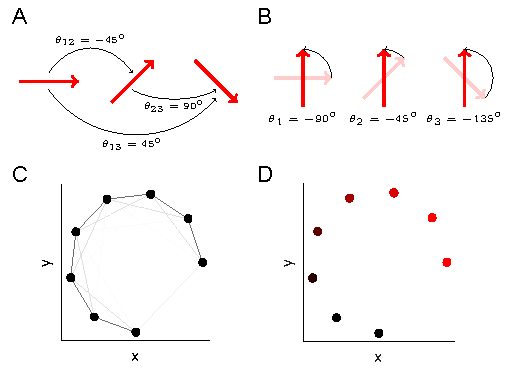
\includegraphics[width=8.7cm]{fig2}
\caption{Schematic illustrating angular synchronization and diffusion maps. {\xfigtextfontit (A)} Set of vectors, each in a different orientation. The pairwise alignment angles are indicated. {\xfigtextfontit (B)} The vectors from {\xfigtextfontit A}, each rotated about their midpoint so that the set is globally aligned. Note that the chosen rotation angles are consistent with the pairwise alignments in {\xfigtextfontit A}: the differences between a pair of angles in {\xfigtextfontit B} is the same as the pairwise angle in {\xfigtextfontit A}. {\xfigtextfontit (C)} Data points (in black) which lie on a one-dimensional nonlinear curve in two dimensions. Each pair of data points is connected by an edge, and the edge weight is related to the Euclidean distance between the points through the diffusion kernel (see {\xfigtextfontit SI Appendix}), so that close data points are connected by dark (``stronger'') edges. {\xfigtextfontit (D)} The data in {\xfigtextfontit C}, colored by the first (non-trivial) eigenvector from the diffusion map computational procedure. The color intensity is monotonic with the arclength, thus parameterizing the curve.}
%\label{fig:schematics}
\customlabel{fig:schematics}{2}
\customlabel{subfig:synch1}{\ref{fig:schematics}{\it A}}
\customlabel{subfig:synch2}{\ref{fig:schematics}{\it B}}
\customlabel{subfig:dmaps1}{\ref{fig:schematics}{\it C}}
\customlabel{subfig:dmaps2}{\ref{fig:schematics}{\it D}}
\end{figure}


\begin{figure*}[t]
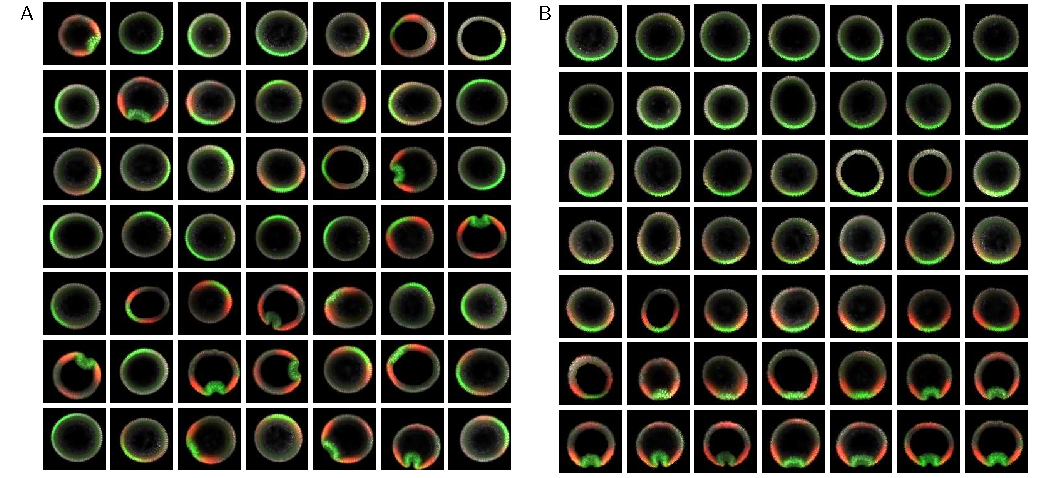
\includegraphics{fig3}
\caption{{\xfigtextfontit Drosophila} during cellularization. {\xfigtextfontit (A)} Images of {\xfigtextfontit Drosophila} embryos collected during cellularization. Each image is of a different embryo in a different rotational and translational orientation. {\xfigtextfontit (B)} Images from {\xfigtextfontit A}, now registered and ordered using vector diffusion maps. The dorsal side of each embryo now appears at the top of each image, and the ventral side appears at the bottom.}
\customlabel{fig:data1}{3}
\customlabel{subfig:raw_data1}{\ref{fig:data1}{\it A}}
\customlabel{subfig:ordered_data1}{\ref{fig:data1}{\it B}}
\customlabel{subfig:averaged_data1}{\ref{fig:data1}{\it C}}
\end{figure*}

\subsection{Images of {\subsectionitfont Drosophila} embryos during cellularization}

As a first illustration of this approach to temporal ordering and registration of images, we analyze a data set where the correct registration and temporal order is known {\it a priori}.
%
This data set is obtained by fluorescent imaging of {\it Drosophila} embryos during the third hour after fertilization.
%
By this stage of development, sequential divisions of the fertilized egg have generated a system where most of the nuclei are arranged in a monolayer under the common plasma membrane \cite{foe1983studies}.
%
Figure~\ref{subfig:raw_data1} shows optical cross-sections of each embryo, with nuclei (gray in the figure) labeled by DAPI, a DNA stain.
%
During the third hour of development, the spatially uniform two-dimensional arrangement of nuclei is patterned by the concentration profiles of chemical signals that control cell differentiation.
%
One of these signals is provided by the nuclear localization of the transcription factor Dorsal (Dl, green in the figure), which subdivides the early embryo into the territories that give rise to the muscle, nerve, and skin tissues.
%
Another signal is provided by the phosphorylated form of the extracellular signal regulated kinase (dpERK, red in the figure), an enzyme that specifies a subset of neuronal cells.
%


%%%YGK say a simple thing in the caption about Dorsal-Ventral

Previous studies \cite{rushlow2012temporal} established that throughout the third hour of development, the nuclear localization of Dl is unimodal and peaked at the ventral side of the embryo (see {\it SI Appendix}).
%
The spatiotemporal pattern of dpERK is more complex: dpERK is first detected in two lateral stripes, which increase in intensity towards the end of the third hour \cite{lim2013kinetics}.
%
This bimodal pattern is then augmented by a peak at the dorsal side of the embryo.
%
Both of these features become readily apparent when images are registered and ordered using vector diffusion maps (see Figure~\ref{subfig:ordered_data1}): the peak of nuclear Dl is consistent throughout the images and intensity of the dpERK signal in the lateral regions of the embryo monotonically increases across the data set.
%

For this data set, the quality of the temporal ordering provided by vector diffusion maps can be assessed by comparing with the ordering obtained through an independent approach.
%
During the third hour of development, the embryo cellularizes: nuclei located under common plasma membrane are enclosed by lateral membranes which grow inward, separating the nuclei into individual cells.
%
The highly reproducible kinetics of lateral membrane growth can be used to estimate the age of each embryo to within 1--3 minutes \cite{figard2013plasma} (see {\it SI Appendix}).
%
Spearman's rank correlation coefficient between the orderings obtained based on the progress of cellularization and vector diffusion maps is 0.91.
%
Thus, we have validated a dimensionality reduction approach to temporal ordering and registration of data on a data set where image orientation and ordering can be assessed independently.

Although the first vector diffusion maps coordinate accurately captures the developmental dynamics, there are other sources of variability within this data set that could also be extracted using these techniques.
%
An obvious one is variability due to size; here, the size variation is relatively small relative to the developmental changes.
%
However, in other applications where the size variation is significant or the developmental dynamics are more subtle, it may be important to factor out size or {\it scaling} symmetries.
%%%
%%%YGK   for teh "additional components" - don't have in the same sentence - say it somewhere else.... INCLUDE IT (maybe in the mutants)


%Furthermore, the dynamics uncovered by vector diffusion maps is relatively simple, which suggests that a simpler approach could have been used to order the data.
%
%Indeed, a principal component analysis (PCA) of registered data reveals that data can be accurately ordered by projecting each image onto the first PCA mode.

\subsection{Images of gastrulating  {\subsectionitfont Drosophila} embryos}

As the images in Figure~\ref{fig:data1} are relatively simple, other techniques could have been used to temporally order them.
%
Because this data set is effectively a single mode (the two dpERK peaks) growing in time,
principal component analysis (PCA) \cite{shlens2005tutorial} would uncover most of the meaningful structure in the data, and projection onto the first principal component would be sufficient to order the data.
%
However, developmental dynamics are often significantly more complex, and nonlinear techniques such as (vector) diffusion maps are required to extract meaningful structure in the data.
%
The next data set illustrates this point.

Figure~\ref{subfig:raw_data2} shows a data set of $108$ images of {\it Drosophila} embryos.
%
These images cover a thirty minute time interval and span late cellularization (the early images in this data set overlap with the late images in the previous set) through gastrulation, when the two-dimensional sheet of newly formed cells begins to deform into three-dimensional structures which will form the future organs.
%
As before, each image is an optical cross-section of an embryo fixed at a different developmental time.
%
The nuclei (gray) are again labeled with a DNA marker.
%
However, during this developmental time period, the nuclei are no longer uniformly arranged around the periphery of the embryo.
%
Instead of Dl, which is difficult to visualize at this point, we stained for Twist (Twi, shown in green), a transcription factor that is activated by high levels of Dl, specifying the cells of the future muscle tissue.
%

%
During this developmental time span, the ventral furrow is formed, where the ventral side of the embryo buckles towards the center of the embryo, bringing in the future muscle cells.
%
dpERK (red) again appears as two lateral peaks at the ventral side of the embryo.
%
These two peaks merge together during invagination, eventually forming (together with Twi) a characteristic ``omega'' shape.
%
During this time window, germband elongation causes cells from the ventral side to move towards the poles of the embryo, and then wrap around to the dorsal side.
%
At the end of this process, cells which were originally on the ventral side have migrated to the dorsal side of the embryo, causing similar ``omega'' shaped patterns (formed by Twi and dpERK) to arise on the dorsal side (shown in the late images in Figure~\ref{subfig:averaged_data2}).

\begin{figure*}[t]
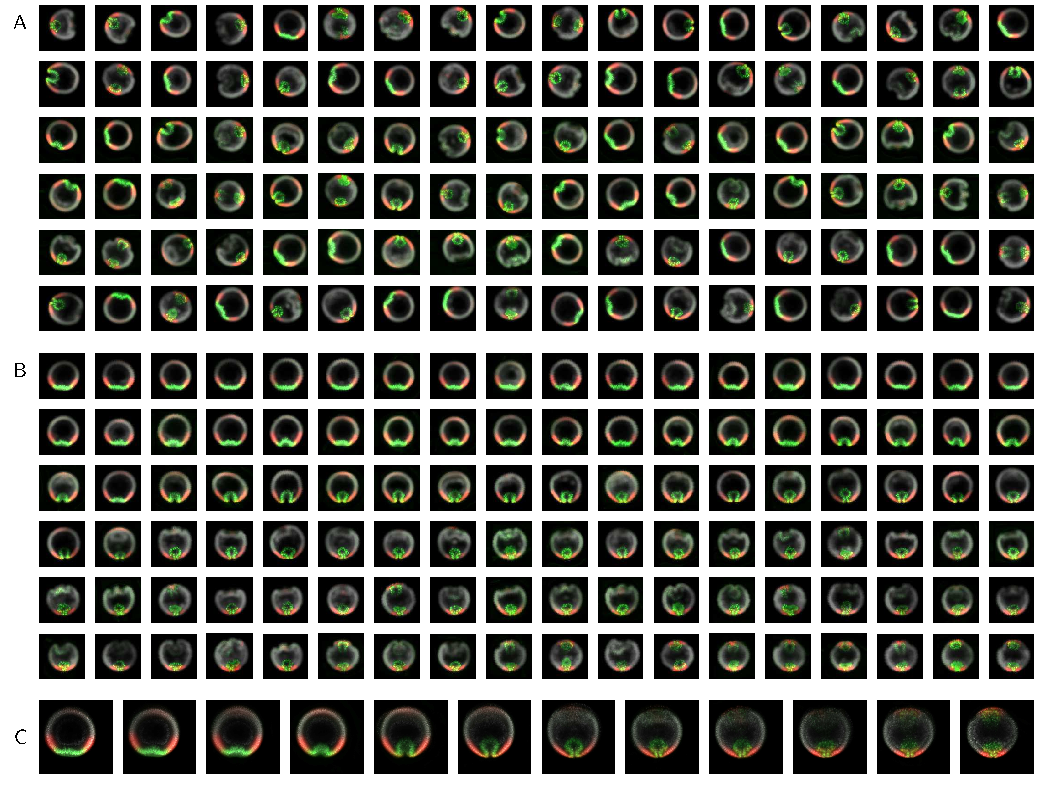
\includegraphics{fig4}
\caption{{\xfigtextfontit Drosophila} during gastrulation. {\xfigtextfontit (A)} Images of gastrulating {\xfigtextfontit Drosophila} embryos. Each image is of a different embryo in a different rotational and translational orientation. {\xfigtextfontit (B)} Data from {\xfigtextfontit A}, registered and ordered using vector diffusion maps. {\xfigtextfontit (C)} Average trajectory of the images shown in {\xfigtextfontit B}. Each image is the average of $9$ consecutive images in {\xfigtextfontit B}. }
\customlabel{fig:data2}{4}
\customlabel{subfig:raw_data2}{\ref{fig:data2}{\it A}}
\customlabel{subfig:ordered_data2}{\ref{fig:data2}{\it B}}
\customlabel{subfig:averaged_data2}{\ref{fig:data2}{\it C}}
\end{figure*}

Visually, the dynamics in this data set are highly nonlinear, and only 22\% of the variability in the data is captured by the first principal component.
%
We require a more sophisticated approach, such as vector diffusion maps, to temporally order the data.
%
Figure~\ref{subfig:ordered_data2} shows the images in Figure~\ref{subfig:raw_data2}, now registered and ordered using vector diffusion maps \cite{singer2012vector}.
%
Visual inspection verifies that this ordering is consistent with the known developmental dynamics outlined above.
%
However, the dynamics are not immediately apparent from this set of registered and ordered images for two reasons.
%
First, the sheer number of images makes visual assimilation of the entire data set (even after registration and ordering) difficult, and
second, the ordered data is not entirely smooth due to noise from interembryo variability.
%
To highlight the developmental dynamics revealed by vector diffusion maps, we construct a movie of an averaged developmental trajectory by applying a Gaussian filter to the set of ordered images (more details are given in the {\it SI Appendix}). 
%
This movie is included in the {\it SI Appendix},
and representative snapshots from this movie are shown in Figure~\ref{subfig:averaged_data2}.
%
The stereotypic dynamics are now readily apparent.
%
However, there are some artifacts in the movie due to size variation, the dynamics at the end of the movie are not as smooth, as we have fewer samples in this time window.
%
We would like to note that, although this movie provides us with a representative picture of the dynamics, the speed of the movie is not constant with time, as we have no true time information about the images.
%
We have thus accomplished the same task presented in the caricature in Figure~\ref{fig:fish}, but without knowledge about the appropriate landmarks (e.g., fins) for registration or the appropriate statistic (e.g., body size) by which to order.

\subsection{Identifying distinct developmental trajectories}

Vector diffusion maps can not only temporally order data, but can also uncover other sources of variability.
%
Up to this point, we have assumed that our experiments contain one main direction of variability, and that this direction is parameterized by time.
%
However, this is not always the case.
%
As an example, we have collected a data set consisting of $42$ embryos undergoing cellularization during the third hour of development (see {\it SI Appendix}); $21$ of the embryos are wild type, and $21$ of the embryos are mutant embryos where dpERK is expressed in one broad peak at the ventral side.
%
Again, each image is an optical cross-section of an embryo fixed at a different developmental time, and the embryos have been stained for nuclei (gray), Dl (green), and dpERK (red).
%
We expect two sources of variability in this data set: differences due to developmental time, and differences between mutant and wild type dynamics.

Figure~\ref{subfig:projection_data3} shows the data, projected onto the first two vector diffusion maps coordinates;
each data point corresponds to one image in our data set.
%
For the previous examples, where we only uncovered developmental progression, we used the first vector diffusion maps coordinate (i.e., the x-axis of this plot) to order the data.
%
However, our data now contains two main sources of variation, and we can see two distinct trajectories, highlighted in blue and red, emerge in this two-dimensional projection.
%
Both curves originate from a common point, and then diverge.
%
Representative images along the blue and red curves are shown in Figures~\ref{subfig:average_wt_data3}~and~\ref{subfig:average_mut_data3}.
%
Figure~\ref{subfig:average_wt_data3}, corresponding to the blue curve, shows the emergence of two distinct dpERK peaks, and Figure~\ref{subfig:average_mut_data3} reveals one more concentrated dpERK peak.
%
This is consistent with previously known dynamics:
at early times, the wild type and mutant embryos both have little dpERK signal, and are therefore indistinguishable, and at later times, the two groups separate as the wild type embryos develop two distinct dpERK peaks and the mutant embryos develop only a single peak.
%
We have therefore shown that vector diffusion maps can not only recover dynamics, but also distinguish different expression patterns and developmental trajectories.

\begin{figure}[t]
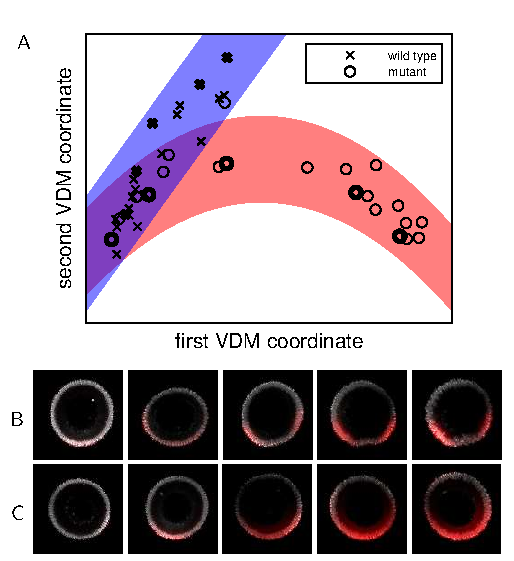
\includegraphics{fig5}
\caption{Mutant and wild type {\xfigtextfontit Drosophila}.  {\xfigtextfontit(A)} Data collected from wild type and mutant embryos (original data set is shown in {\xfigtextfontit SI Appendix}), projected onto the first two vector diffusion maps coordinates. The two distinct trajectories are highlighted in blue and red. {\xfigtextfontit (B)} dpERK signal at select wild type points in {\xfigtextfontit A} (denoted by bold symbols). {\xfigtextfontit (C)} dpERK signal at select mutant points in {\xfigtextfontit A} (denoted by bold symbols).}
\customlabel{fig:data3}{5}
\customlabel{subfig:projection_data3}{\ref{fig:data3}{\it A}}
\customlabel{subfig:average_wt_data3}{\ref{fig:data3}{\it B}}
\customlabel{subfig:average_mut_data3}{\ref{fig:data3}{\it C}}
\end{figure}

%\begin{figure*}[t]
%\raisebox{8cm}{{\figtextfont A}}
%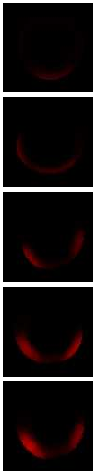
\includegraphics[height=8.4cm]{wt_trajectory2}
%%\raisebox{8cm}{{\figtextfont B}}
%\begin{tikzpicture}
%     \node at (0,0)
%       {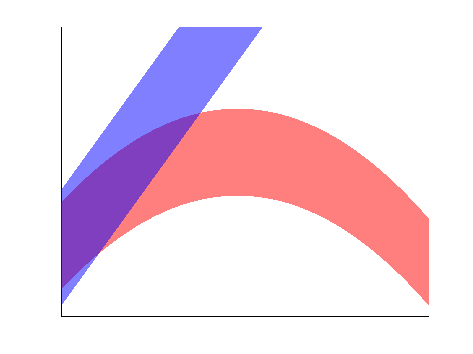
\includegraphics[height=8.4cm]{mut_wt_vdm_embedding_background}};
%     \node at (0,0)
%       {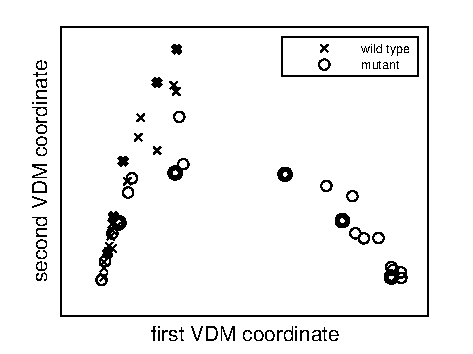
\includegraphics[height=8.4cm]{mut_wt_vdm_embedding}};
%     \node at (-5cm, 3.8cm)
%       {{\figtextfont B}};
%\end{tikzpicture}
%\raisebox{8cm}{{\figtextfont C}}
%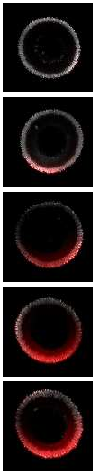
\includegraphics[height=8.4cm]{mut_trajectory2}
%\caption{Mutant and wild type {\xfigtextfontit Drosophila}.  {\xfigtextfontit (A)} dpERK signal at select wild type points in {\xfigtextfontit B} (denoted by bold symbols). {\xfigtextfontit(B)} Data collected from wild type and mutant embryos (original data set is shown in {\xfigtextfontit SI Appendix}), projected onto the first two vector diffusion maps coordinates. The two distinct trajectories are highlighted in blue and red. {\xfigtextfontit (C)} dpERK signal at select mutant points in {\xfigtextfontit B} (denoted by bold symbols).}
%\customlabel{fig:data3}{5}
%\customlabel{subfig:average_wt_data3}{\ref{fig:data3}{\it A}}
%\customlabel{subfig:projection_data3}{\ref{fig:data3}{\it B}}
%\customlabel{subfig:average_mut_data3}{\ref{fig:data3}{\it C}}
%\end{figure*}

\section{Conclusions}

We have demonstrated how vector diffusion maps, an existing reduction technique, can be used to register and temporally order images from developmental biology studies.
%
We acknowledge that the tasks of both registration and ordering could have been accomplished using a variety of other techniques.
%
We chose the algorithm outlined here, not because it is specifically tailored to our particular data sets, but rather, because it is sufficiently general and we are confident that it can be applied to a myriad of biological imaging applications.
%
Furthermore, such data mining algorithms are often tested on databases containing hundreds or thousands of images.
%
Here, we could successfully recover the underlying dynamics with relatively small data sets.
%
In general, the number of images required to accurately recover the dynamics will be a function of the noise in the data, as well as the dynamic range and complexity of the underlying process.

The task of image registration has been widely studied \cite{zitova2003image}, for applications such as face recognition \cite{rowley1998rotation}, medical image registration \cite{hajnal2010medical}, and texture classification \cite{greenspan1994rotation}.
%
However, most of these applications rely on the definition and identification of good landmarks or features within each image.
%
For example, in face recognition, the first step is often to locate the eyes, nose, and mouth in each face, and then register images by aligning these features \cite{zhao2003face}.
%
%Temporally ordering images of a construction site over time is also based on first identifying features within the images \cite{schindler2007inferring}.
%
Because of the complexity of chemical and morphological changes in developing tissues, appropriate features may not be known {\it a priori}.
%
We therefore use an algorithm which requires no features, but instead, uses only the raw pixel images and the inherent geometric symmetry of the problem.
%
%Template-based methods are also common for registration, where one optimally aligns each image to a predefined template function.
%
%However, these methods can suffer when the images are noisy, and the success of such methods can depend strongly on the template function \cite{shatsky2009method}.
%

The task of temporal ordering has also been studied in a variety of biological applications.
%
Data sets such as transcriptional profiling data (where each data point is the transcriptome for a single sample, such as a cell or tissue sample from a patient) \cite{anavy2014blind, trapnell2014dynamics,gupta2008extracting, qiu2011discovering} and snapshots of cells throughout the cell cycle (where each point is a vector of features, such as the amount of DNA, which quantify the cell's state)  \cite{kafri2013dynamics} have been temporally ordered to extract representative trajectories of the underlying dynamic processes.
%
Many of these applications order the data by solving a traveling salesman problem (TSP) or constructing a minimum spanning tree (MST) on the data,
expecting that these structures (the path of the traveling salesman, or the minimum spanning tree) characterize the majority of the patterns and variability within the data and provide an accurate encoding of the dynamical progression.
%
These algorithms often use dimensionality reduction techniques (typically PCA or variants of) as a preprocessing step.
%
The TSP or MST is solved/constructed not in the original data space, but rather in the lower-dimensional space of the first few principal components.
%
In these approaches, PCA serves two purposes: it denoises the data, making the TSP/MST construction more robust, and also allows for easy visualization of the TSP/MST if one only uses the first two or three principal components.

We, instead, use vector diffusion maps to construct a one-dimensional parameterization of the data.
%
Because vector diffusion maps is a dimensionality reduction technique, it serves as a denoising step and yields smooth averaged trajectories even under noisy conditions.
%
However, because the algorithm is nonlinear, it affords us many of the same geometric flexibilies as the MST or TSP formulations.
%
Vector diffusion maps are one of many nonlinear dimensionality reduction techniques that have been recently developed \cite{Belkin2003, tenenbaum2000global, Donoho2003, Roweis2000}.
%
Diffusion maps have been shown to be more robust to noise than isomap \cite{balasubramanian2002isomap}, a path-based algorithm, and so we suspect the methods presented here may perform better than the ordering algorithms used in previous work.

Furthermore, dimensionality reduction techniques such as vector diffusion maps do not constrain us to one-dimensional parameterizations/organizations of the data, as illustrated in the mutant data set example (Figure~\ref{fig:data3}).
%
These techniques would also allow us to compare the developmental dynamics of several different mutations to see how mutations are developmentally related.
%
Other sources of variability, such as size or viewing angle, could also be uncovered using vector diffusion maps.

After registering and temporally ordering images, one can perform a variety of post-processing tasks to gain further insight into the developmental processes.
%
We have demonstrated one such technique (Gaussian filtering) that allows us to extract a more representative developmental trajectory from the set of noisy snapshots.
%
%Constructing a smooth movie from the registered and ordered cross-sectional snapshots would also be of biological interest, and
Examining the top principal components in different time windows would allow one to visualize the main dynamical features along the trajectory.
%
%These questions first require that the data be registered and temporally ordered.
%
Correlating vector diffusion maps coordinates with physical variables is another post-processing task that can give physical insight into developmental dynamics.
%
One can test which physical variable, among a set of candidate physical variables (e.g., total intensity of one signal, roundness of the embryo), is most correlated with the uncovered vector diffusion maps coordinate to help understand which physical quantities change across the developmental trajectory.
%
We are confident that, as biological becomes easier and more robust, the dimensionality reduction techniques we present here will play an important role in the data analysis pipeline.


\begin{itemize}
\item What are other people doing  (maybe critically)
\item Movies  smoothness
\item Discrete symmetries like flips
\item Local information ? (features of the image) (associate with Fourier-Bessel and bispectra)
\item Mutant-wildtype stuff  IMPORTANT
\item And in general, MULTIPLE variablities is important (mutants, guys in another cycle, etc.)

%\item size is an issue
\item  small tilts is an issue
\item   could one do three-d image processing ?  of the floating thing, without the device
\item how do we go about merging data sets ?
\end{itemize}

%% == end of paper:

%% Optional Materials and Methods Section
%% The Materials and Methods section header will be added automatically.

%% Enter any subheads and the Materials and Methods text below.


\begin{materials}


\end{materials}


%% Optional Appendix or Appendices
%% \appendix Appendix text...
%% or, for appendix with title, use square brackets:
%% \appendix[Appendix Title]


\begin{acknowledgments}
- text of acknowledgments here, including grant info -
\end{acknowledgments}

%% PNAS does not support submission of supporting .tex files such as BibTeX.
%% Instead all references must be included in the article .tex document.
%% If you currently use BibTeX, your bibliography is formed because the
%% command \verb+\bibliography{}+ brings the <filename>.bbl file into your
%% .tex document. To conform to PNAS requirements, copy the reference listings
%% from your .bbl file and add them to the article .tex file, using the
%% bibliography environment described above.

%%  Contact pnas@nas.edu if you need assistance with your
%%  bibliography.

% Sample bibliography item in PNAS format:
%% \bibitem{in-text reference} comma-separated author names up to 5,
%% for more than 5 authors use first author last name et al. (year published)
%% article title  {\it Journal Name} volume #: start page-end page.
%% ie,
% \bibitem{Neuhaus} Neuhaus J-M, Sitcher L, Meins F, Jr, Boller T (1991)
% A short C-terminal sequence is necessary and sufficient for the
% targeting of chitinases to the plant vacuole.
% {\it Proc Natl Acad Sci USA} 88:10362-10366.


%% Enter the largest bibliography number in the facing curly brackets
%% following \begin{thebibliography}

\bibliographystyle{pnas}
\bibliography{background_reading/references,../../references/references}

%\begin{thebibliography}{}

%\end{thebibliography}


\end{article}

\end{document}


